%%%%%%%%%%%%%%%%%%%%%%%%%%%%%%%%%%%%%%%%%
% MOST Report for 2014
% CERN working period: 10/9 - 28/10
% Edit by Jun-Yi Wu
%%%%%%%%%%%%%%%%%%%%%%%%%%%%%%%%%%%%%%%%%

%----------------------------------------------------------------------------------------
%	PACKAGES AND OTHER DOCUMENT CONFIGURATIONS
%----------------------------------------------------------------------------------------

\documentclass[12pt]{article} % Default font size is 12pt, it can be changed here
\usepackage{geometry} % Required to change the page size to A4
\geometry{a4paper} % Set the page size to be A4 as opposed to the default US Letter
\usepackage{graphicx} % Required for including pictures
\usepackage{float} % Allows putting an [H] in \begin{figure} to specify the exact location of the figure
\usepackage{wrapfig} % Allows in-line images such as the example fish picture
\linespread{1.2} % Line spacing
\setlength\parindent{2em} % Uncomment to remove all indentation from paragraphs
\setlength{\parskip}{1em}
\graphicspath{{figure/}} % Specifies the directory where pictures are stored
\setlength{\oddsidemargin}{0pt}
\setlength{\textwidth}{460pt}
\setlength{\textheight}{660pt}
\usepackage{chngcntr}
\usepackage{hyperref}
\counterwithin{figure}{section}
\counterwithin{table}{section}
\newcommand{\tabincell}[2]{\begin{tabular}{@{}#1@{}}#2\end{tabular}} 
\usepackage{caption}

\begin{document}

%----------------------------------------------------------------------------------------
%	TITLE PAGE
%----------------------------------------------------------------------------------------

\begin{titlepage}

  \newcommand{\HRule}{\rule{\linewidth}{0.5mm}} % Defines a new command for the horizontal lines, change thickness here

  \center % Center everything on the page

  \textsc{\LARGE National Center University}\\[1.5cm] % Name of your university/college
  \textsc{\Large Department of Physics}\\[0.5cm] % Major heading such as course name
  \textsc{\large MOST Report 2014}\\[0.5cm] % Minor heading such as course title

  \HRule \\[0.4cm]
         { \huge \bfseries Study of XtoZH and Validation of aMC@NLO}\\[0.4cm] % Title of your document
         \HRule \\[1.5cm]

         \begin{minipage}{0.4\textwidth}
           \begin{flushleft} \large
             \emph{Author:}\\
             Wu \textsc{Jun-Yi} % Your name
           \end{flushleft}
         \end{minipage}
         ~
         \begin{minipage}{0.4\textwidth}
           \begin{flushright} \large
             \emph{Supervisor:} \\
             Yu \textsc{Shin-Shan} % Supervisor's Name
           \end{flushright}
         \end{minipage}\\[4cm]

         {\large \today}\\[3cm] % Date, change the \today to a set date if you want to be precise

         %\includegraphics{Logo}\\[1cm] % Include a department/university logo - this will require the graphicx package

         \vfill % Fill the rest of the page with whitespace

\end{titlepage}


%----------------------------------------------------------------------------------------
%	TABLE OF CONTENTS
%----------------------------------------------------------------------------------------

\tableofcontents % Include a table of contents

\newpage % Begins the essay on a new page instead of on the same page as the table of contents 


%----------------------------------------------------------------------------------------
%	INTRODUCTION
%----------------------------------------------------------------------------------------

\section{Introduction} % Major section

In this report, we introduce some steps for searching a TeV resonances going to ZH final states. We will introduce some jet selections. These selections are kept voluntarily loose in order not to depend too much on the nature of the TeV resonance. In particular, the Z boson is selected leptonically (with electron or muon final state) while the Higgs is chosen to decay fully hadronically ($q\bar{q}$ merge into jet).

Despite the small final branching ratio, this channel is found to be a reasonable compromise between a strong signature and an acceptable statistics. The two leptons are easily identified by the detector and limit the presence of the background, while the hadronic Higgs decay collects the largest possible fraction of Higgs events. 

We also introduce the validation of new and old signal Monte Carlo models, the new model will be used in the future analysis. Before that, we need to make sure the basic kinematics are the same as what we use now. 

The another part of this report is validation of new and old matrix element generators, we will look at some basic kinematic plots.


\newpage


%----------------------------------------------------------------------------------------
%	MAJOR SECTION 1
%----------------------------------------------------------------------------------------

\section{Pre-selection} % Major section

As a fundamental step of the analysis, we need to check the accuracy of the MC simulation and allows us to study in detail the physical process under consideration. In this section, the selection criteria of jet are discussed, then all relevant data and MC distributions are shown.


\subsection{Jet requirements} % Sub-section

Jets are clustered from the list of Particle Flow (PF) candidates that are reconstructed in the event.Charged hadrons originating from vertices other than the primary vertex are not used in the jet clustering procedure. In this analysis the CA8 (Cambridge-Aachen) algorithm with a cone radius of $R$ = 0.8 is used for the identification of jets and jet candidates are selected with $p_T$ $>$ 30 GeV and $\left|\eta\right|$ $<$ 2.4. Furthermore jets are required to pass the following loose identificationcriteria:


\noindent
$\bullet$ muon energy fraction smaller than 0.99 \\
$\bullet$ photon energy fraction smaller than 0.99 \\
$\bullet$ charged electromagnetic energy fraction smaller than 0.99 \\
$\bullet$ neutral hadron energy fraction smaller than 0.99 \\
$\bullet$ charged hadron energy fraction larger than 0 \\
$\bullet$ number of constituent particles larger than 1. 


\subsection{Pre-selection of MC signal and background} % Sub-section

In this section all the control plots at the pre-selection level are presented. Table~\ref{tab:selection} reports a summary of the pre-selection requirement described in the above sections. Figure~\ref{fig:MuEF} Figure~\ref{fig:PhoEF} Figure~\ref{fig:CEmEF} Figure~\ref{fig:NHadEF} Figure~\ref{fig:CHadEF} These plots present the ID variables for the jet selections, which are introduced in the previous section. And these distributions are compared between data and MC after N-1 cuts. (for example, plot muon energy fraction without MuEF cut, but still apply cuts to other four variables.) The data and MC comparison generally presents a fair agreement. 


\begin{figure}[H] % Image
  \center{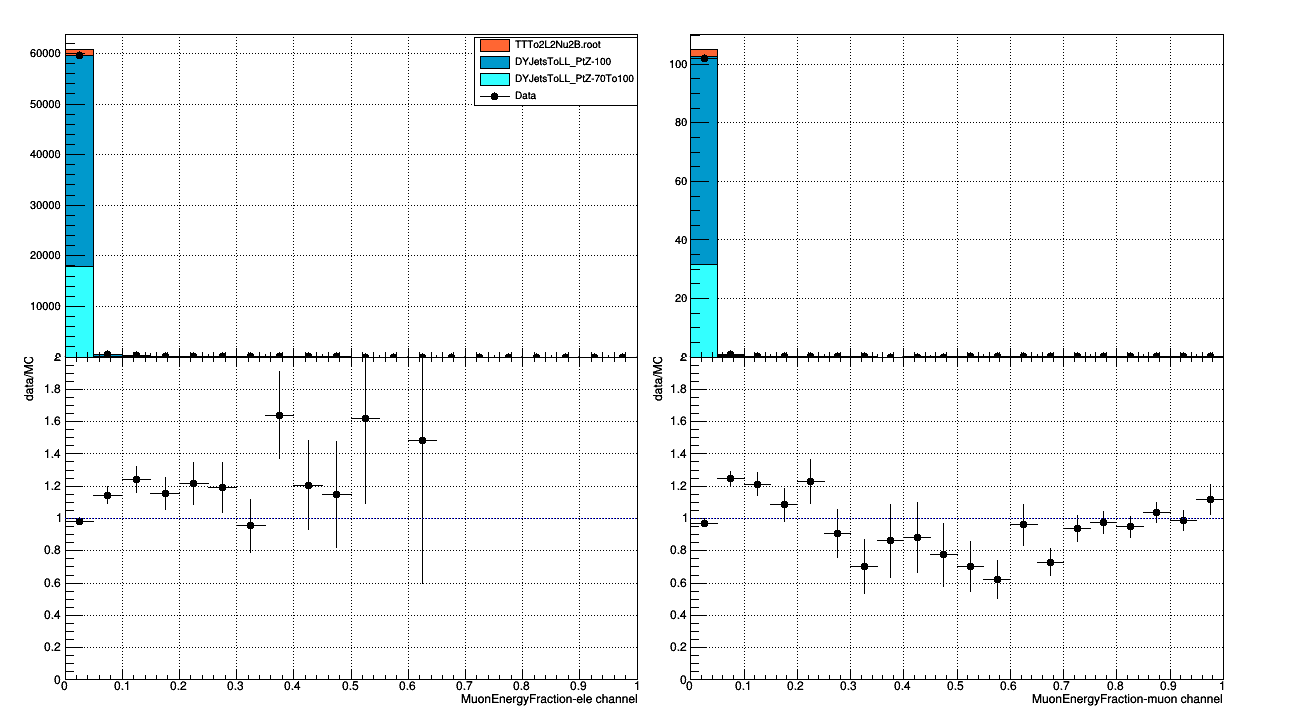
\includegraphics[width=1\linewidth]{h_CA8jetMuEF.png}}
  \caption{Muon energy fraction for two channels. Left: electron channel; Right: muon channel. The definition of muon energy fraction is the muon energy divided by PF jet energy.}
  \label{fig:MuEF}
\end{figure}

\begin{figure}[H] % Image
  \center{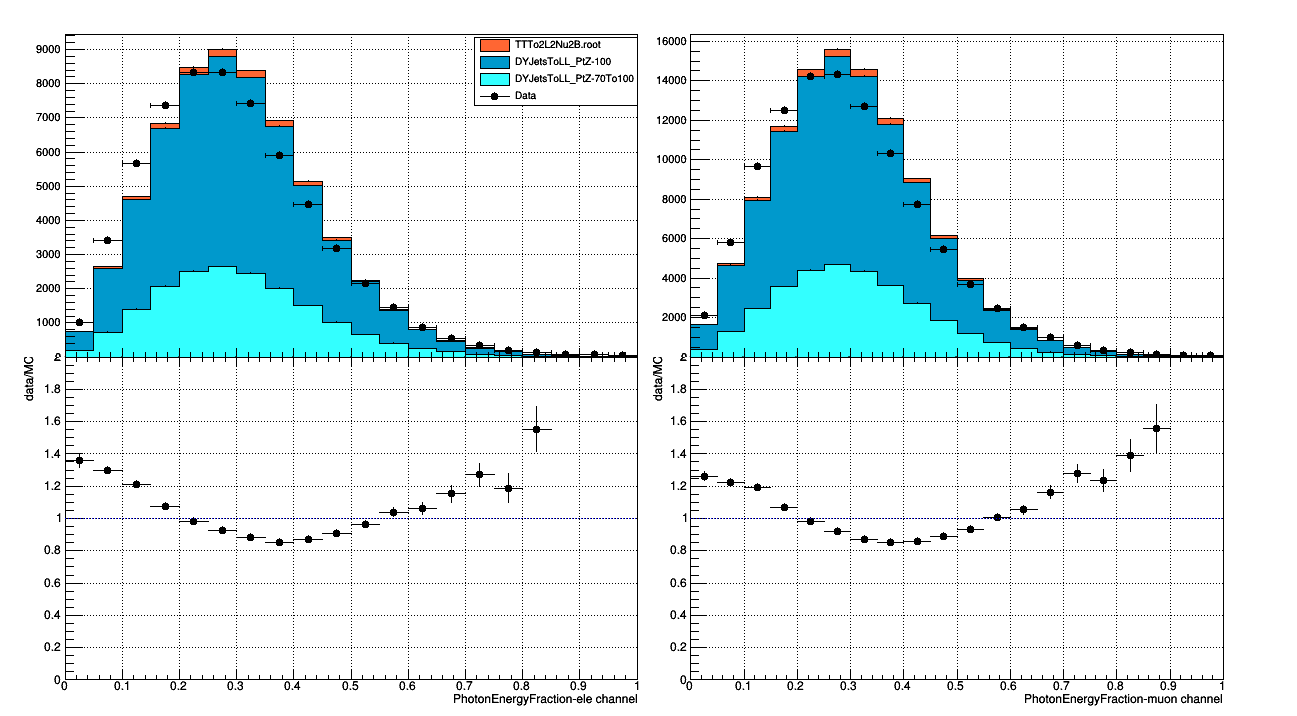
\includegraphics[width=1\linewidth]{h_CA8jetPhoEF.png}}
  \caption{Photon energy fraction for the two channels. Left: electron channel; Right: muon channel. Photon energy fraction is defined by the ratio of photon and PF jet energy.}
  \label{fig:PhoEF}
\end{figure}

\begin{figure}[H] % Image
  \center{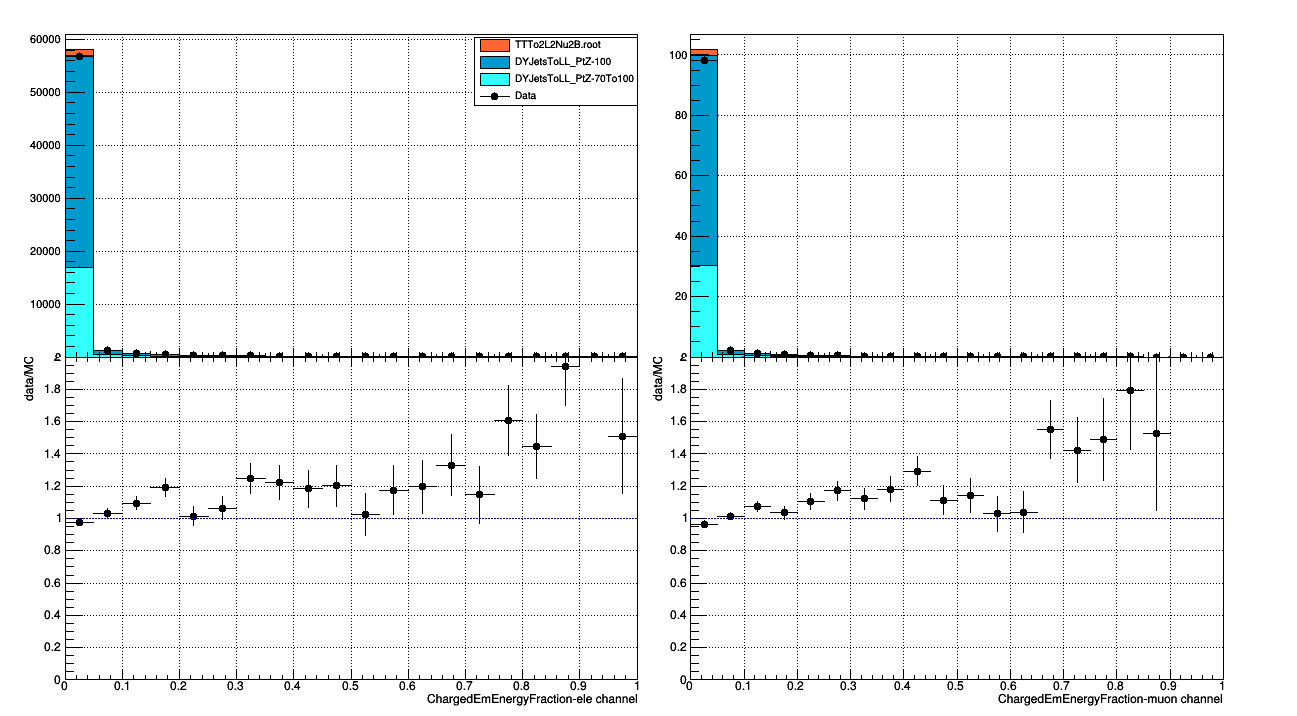
\includegraphics[width=1\linewidth]{h_CA8jetCEmEF.png}}
  \caption{Charged electromagnetic energy fraction for the two channels. Left: electron channel; Right: muon channel. The definition of Charged electromagnetic energy fraction is the energy of charged particles in ECAL divided by PF jet energy.}
  \label{fig:CEmEF}
\end{figure}

\begin{figure}[H] % Image
  \center{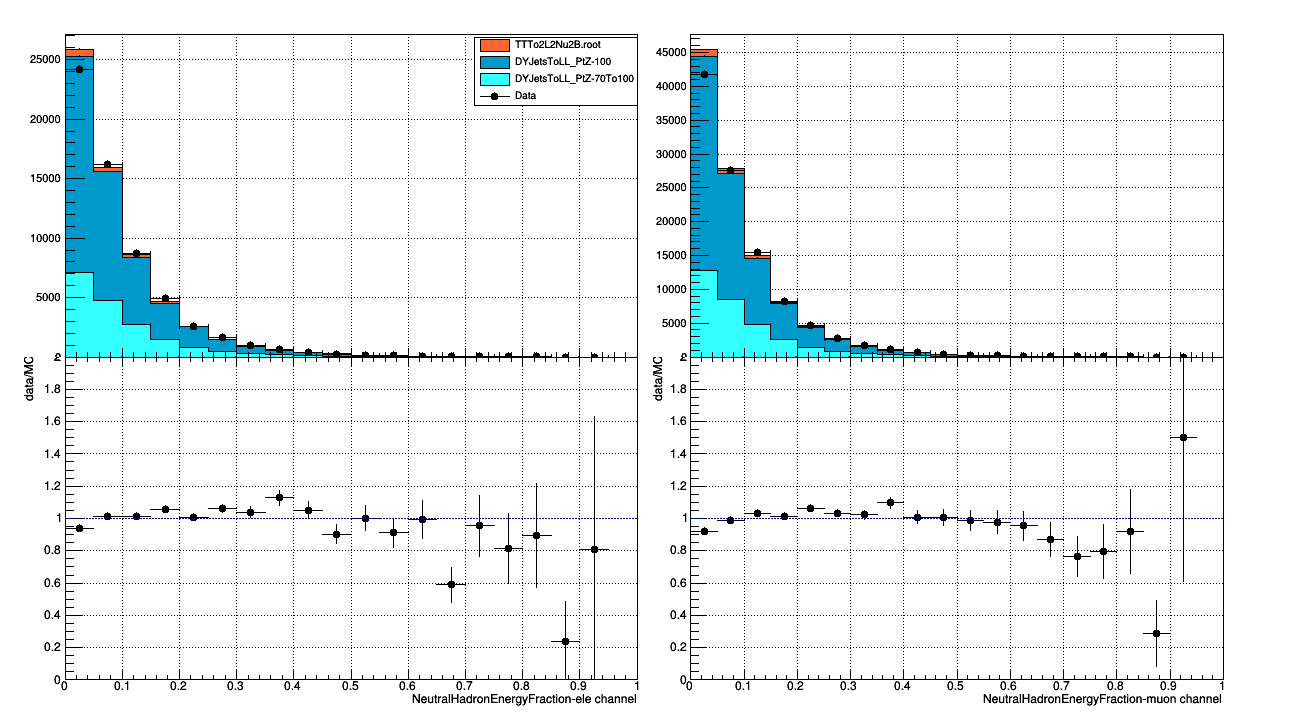
\includegraphics[width=1\linewidth]{h_CA8jetNHadEF.png}}
  \caption{Neutral hadron energy fraction which is defined by the ratio of the energy of neutral particles in ECAL and PF jet energy. For the two lepton dacay channels. Left: electron channel; Right: muon channel.}
  \label{fig:NHadEF}
\end{figure}

\begin{figure}[H] % Image
  \center{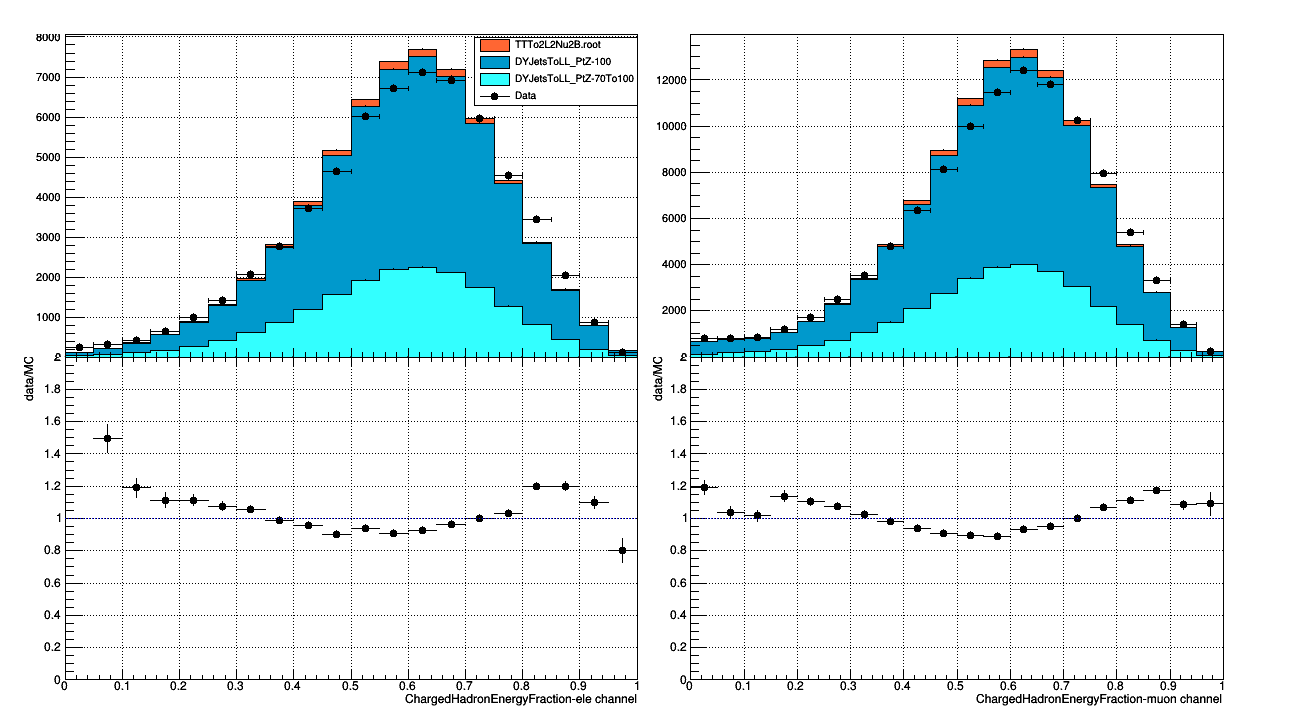
\includegraphics[width=1\linewidth]{h_CA8jetCHadEF.png}}
  \caption{Charged hadron energy fraction for the two lepton decay channels. Left: electron channel; Right: muon channel. The definition of CHadEF is the enery of charged particles in HCAL divided by PF jet energy.}
  \label{fig:CHadEF}
\end{figure}




\begin{center}
  \begin{tabular}{ c c c }
    \hline
    \bf Selection &
    \bf Value &
    \bf Comments \\
    \hline
    Trigger & & \\ \cline{1-1}
    & HLT\_Mu22\_TkMu8 & DoubleMuon dataset \\
    & HLT\_DoubleEle33 & DoublePhoton dataset \\ \hline
    Lepton selections & & \\ \cline{1-1}
    Leading lepton $p_T$ & $p_T$ $>$ 40 GeV & Same for electrons and muons \\ 
    Subleading lepton $p_T$ & $p_T$ $>$ 40 GeV & For electrons \\ 
    Subleading lepton $p_T$ & $p_T$ $>$ 20 GeV & For muons \\ 
    Muon $\eta$ & $\left|{\eta}\right|$ $<$ 2.4 &  \\
    Electron $\eta$ & $\left|{\eta}\right|$ $<$ 2.5 & Avoid the ECAL gap \\
    Electron fiducial & $\left|{\eta}\right|$ out of [1.4442, 1.566] &  \\ \cline{1-1}
    Muon ID & High $p_T$ &  \\
    Muon Isol. $I^{mod}_{trkrel}$ & $<$ 0.1 &  \\ \cline{1-1}
    Electron ID & &  \\
    Ele. Isol. & &  \\
    $I^{mod}_{trk}$ & $<$ 5 GeV &  \\
    $I^{mod}_{HCAL}$ + $I^{mod}_{ECAL}$ & $<$ 2 GeV + 0.03 $E_T$ & EB electrons \\
    & $<$ 2.5 GeV & EE ele. with $E_T$ $<$ 50 GeV \\
    & $<$ 2.5 GeV + 0.03 $E_T$ & EE ele. with $E_T$ $>$ 50 GeV \\ \hline
    Jet selections & & \\  \cline{1-1}
    Jet ID & Loose working point & \\
    Jet $p_T$ & $p_T$ $>$ 30 GeV & \\
    Jet $\eta$ & $\left|{\eta}\right|$ $<$ 2.4 & \\ \hline
    Boson selections & & \\  \cline{1-1}
    $m_{LL}$ & 70 $<$ $m_{LL}$ $<$ 110 GeV & \\
    $m_{J}$ & $m_{J}$ $>$ 40 GeV & \\
    Z $p_T$ & $p_T$ $>$ 80 GeV & \\
    H $p_T$ & $p_T$ $>$ 80 GeV & \\
    \hline
  \end{tabular}
  \captionof{table}{Pre-selection requirements used in the analysis.}
  \label{tab:selection}
\end{center}


\newpage


%----------------------------------------------------------------------------------------
%	MAJOR SECTION 2
%----------------------------------------------------------------------------------------

\section{Final Selection} 

At this section, we study two poweful varialbes that will be introduced later, pruned jet mass and $\tau_{21}$. Then make the appropriate cut on these varibles to discriminate background and signal.

\subsection{Pruned jet mass}

The jet mass is the main observable in distinguishing a H-jet from a QCD jet. Jet pruning consists in the suppression of uncorrelated UE/PU (un-derlying event and pile-up) radiation from the target jet and improves the discrimination pushing the jet mass for QCD jets towards lower values while mantaining the jet mass for V(H)-jets around the boson-mass.

Pruning algorithm is to take a jet of interest and then to recluster it using a vetoed sequential clustering algorithm. Clustering proceeds is vetoed if the particles are too far away in $\Delta$$R$

$\Delta$$R_{ij} > D_{cut} = $$\alpha$$\frac{M_{J}}{P_{T_{J}}}$

and the energy sharing is too asymmetric

$z_{ij} = \frac{P_{T_{i}},P_{T_{j}}}{P_{T_{i+j}}} < z_{cut}$

where z cut and α are parameters of the algorithm. If both these conditions
are satisfied the softer of the two particles is not considered.


\subsection{N-subjettiness}

In order to further discriminate signal from background, it useful to inves-tigate the inner structure of the jet. Studying the distribution of the jet constituents with respect to the jet axis allows us to test the hypothesis of the existence of multiple substructures, that could be evidence of jets originated by more than one parton. This procedure proceeds as follows: the costituents of the jet are clustered again with the usual algorithm, however the procedure is stopped when one obtains N subjets. Then, a new variable, the N-subjettiness, is introduced. It is defined as

$\tau_{N} = \frac{1}{d_{0}}\sum_{k=1}^{}{min((\Delta R_{1,k})^\beta, (\Delta R_{2,k})^\beta ... (\Delta R_{N,k})^\beta})$

where $\beta$ is an arbitrary parameter, the index $k$ runs over the jet constituents and the distances $\Delta R_{N,k}$ are calculated with respect to the axis of the $N^{th}$ subjet. The normalization factor $d_{0}$ is calulated as $d_{0} = \sum_{k}{P_{T,k}\Delta R^{\beta}_{0}}$, setting $R_{0}$ to the radius of the original jet.

In this analysis the N-subjettiness is calculated from the ungroomed jet with the parameter $\beta$ = 1. Let’s now write explicitly the subjettiness relateto the one and two subjet hypothesis,

$\tau_{1} = \frac{1}{d_{0}}\sum_{k}{P_{T,k}\Delta R_{k}}$  and  $\tau_{2} = \frac{1}{d_{0}}\sum_{k}{P_{T,k}min(\Delta R_{1,k},\Delta R_{2,k})}$

In principle, these two quantities should allow us to distinguish the dipole-like nature of the showering of the Higgs decay from the classic monopole structure of QCD jets. In particular, the variable that best discriminates between H-jets and QCD jets is the ratio of 2-subjettiness and 1-subjettiness,

$\tau_{21} = \frac{\tau_{1}}{\tau_{2}}$



\subsection{Signal region} % Sub-section
 
The most discriminating tool to separate signal from the dominant background is the requirement on the pruned mass of the jet. In this analysis the pruned mass of the jet is required to be in the range [110, 140] GeV in order to pass the final selection. The range is chosen in order to contain as much signal as possible without overlapping the signal region of this analysis with other searches of new resonances.

Figure~\ref{fig:fitZpMass} shows the signal region superimposed on the pruned mass ratio distribution. The gaussian fit on the peak of the distribution has as output parameters a mean value around 0.97 and $\sigma$ around 0.056. The difference of the peak mass respect to the real value of the Higgs mass is due to the pruning algorithm applied to the jet, that reduces its reconstructed mass.

\begin{figure}[H] % Image
  \center{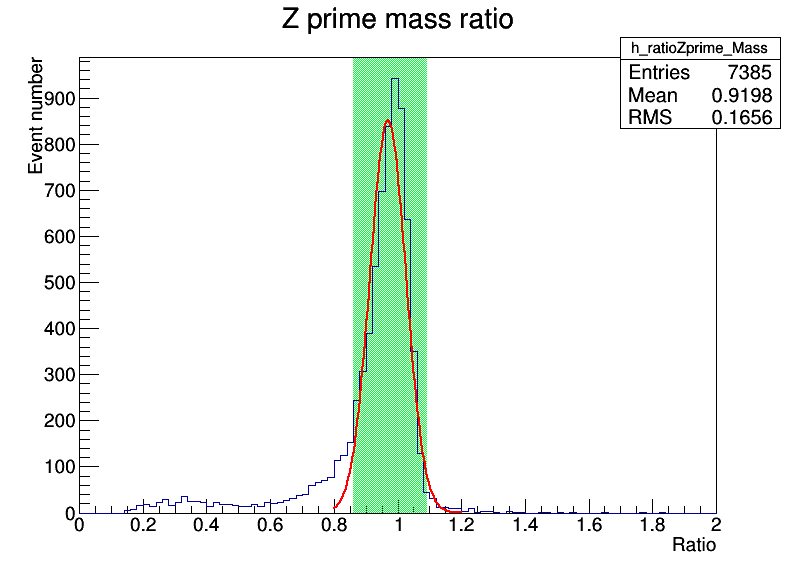
\includegraphics[width=0.8\linewidth]{fitZpMass.png}}
  \caption{Jet pruned mass distribution for a MC signal of 1000 GeV whose peak is fitted with a gaussian function. The signal region is painted in green.}
  \label{fig:fitZpMass}
\end{figure}



\subsection{$\tau_{21}$ cut optimization} % Sub-section

After the selection on the pruned mass, the discriminating power of the ratio $\tau_{21}$ , is reduced since the mass cut and $\tau_{21}$ cut are correlated. In this section we want to study the performances of the selection on this variable.
\\
Optimization procedure: For each mass point we want to establish which is the best value of the $\tau_{21}$ ratio to discriminate signal from background. The procedure is implemented as follows:
\\
\noindent
$\bullet$ set a window of 15\% around the signal resonance mass \\
$\bullet$ plot the expected $\tau_{21}$  variable or signal and background, for the eventsthat passed all the other selection requirements; \\
$\bullet$ integrate the expected $\tau_{21}$ distributions of signal and background up max . The values obtained are an estimation of the to a threshold $\tau_{21}$ max point. The values obtained are an estimation of the signal selection efficiency and the amount of background; \\
This procedure is repeated for values of $\tau_{21}$ ranging form 0.05 to 0.95 in steps of 0.05. In figures Figure~\ref{fig:tau21_M1000} Figure~\ref{fig:tau21_M1500} Figure~\ref{fig:tau21_M2000} the results of the optimiza-tion procedure for signal of 1000, 1500 and 2000 GeV are reported.

And here are the definition of significance and efficiency.

$\bullet$ Efficiency: number of events passing certain $\tau_{21}$ upper threshold divided by the number of events before $\tau_{21}$ cut.

$\bullet$ Significance: $\frac{EFF_{signal}}{1.0+sqrt(B)}$ , numerator is signal efficiency while B is the number of background events passing certain threshold  \\
\\
\\


\begin{figure}[H] % Image
  \center{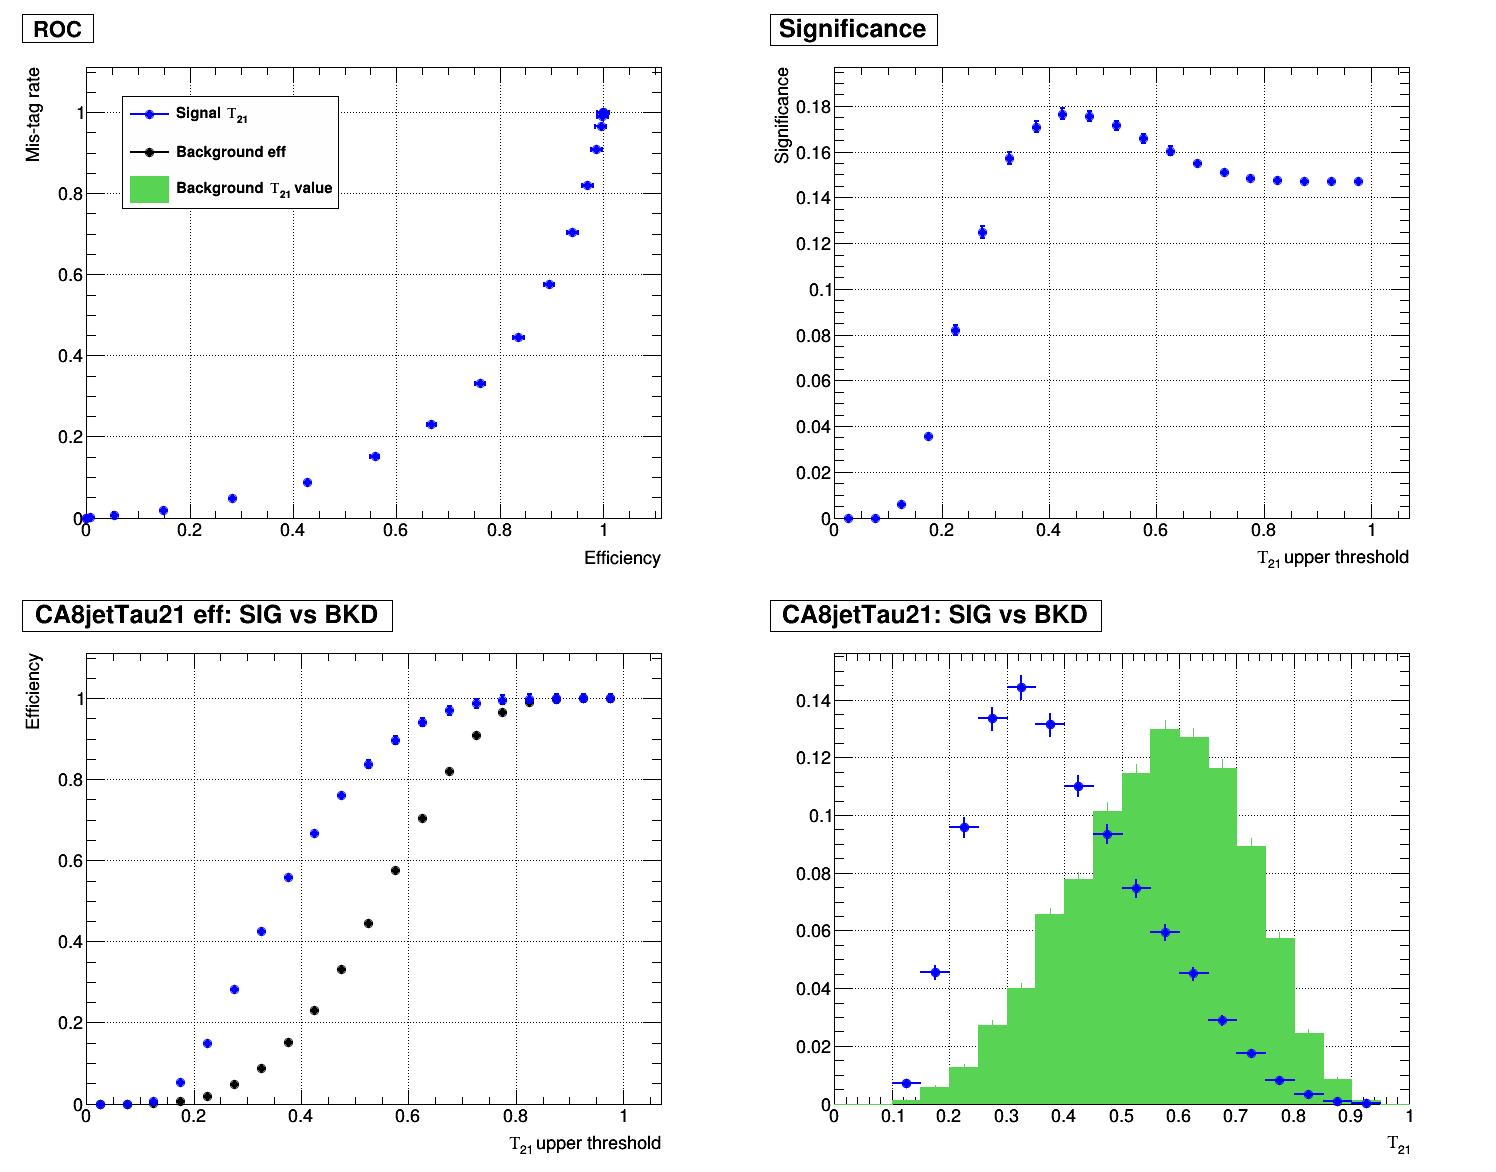
\includegraphics[width=0.8\linewidth]{tau21_M1000.png}}
  \caption{ZPrime mass 1000 GeV - upper left: ROC plot ; upper right: signal significance ; lower left: signal efficiency vs mistag rate ; lower rigth: compare $\tau_{21}$ distribution between MC signal and background}
  \label{fig:tau21_M1000}
\end{figure}

\begin{figure}[H] % Image
  \center{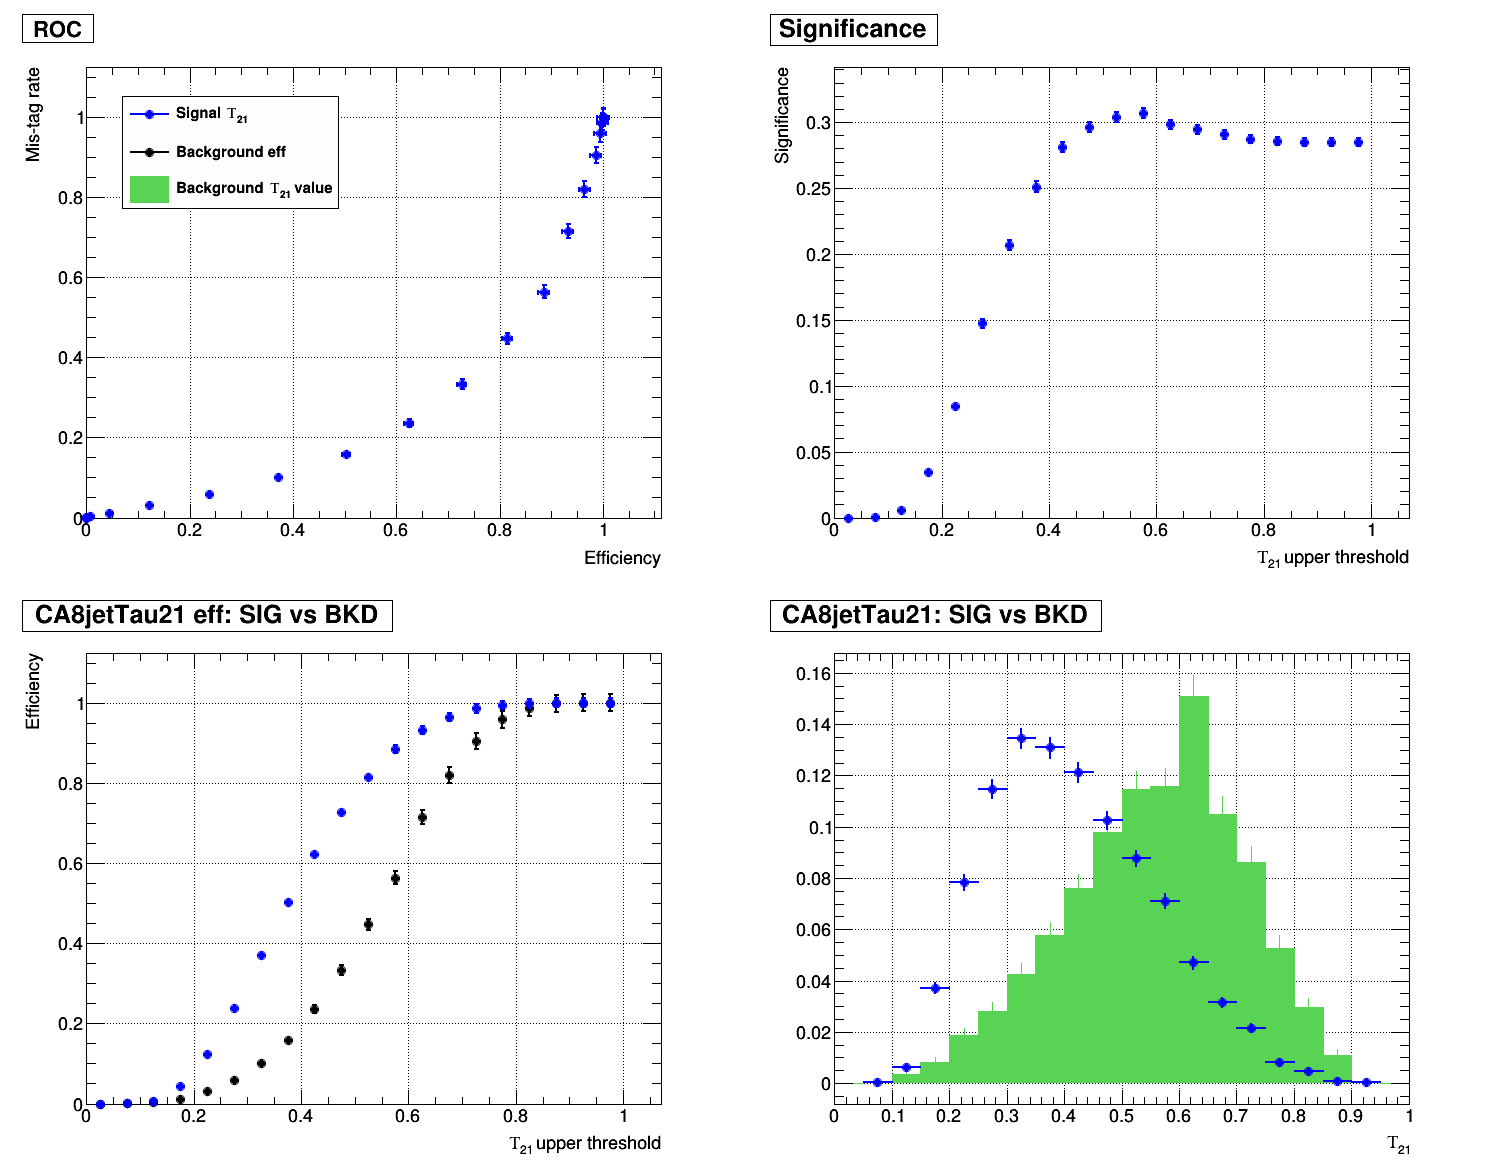
\includegraphics[width=0.8\linewidth]{tau21_M1500.png}}
  \caption{ZPrime mass 1500 GeV - upper left: ROC plot ; upper right: signal significance ; lower left: signal efficiency vs mistag rate ; lower rigth: compare $\tau_{21}$ distribution between MC signal and background}
  \label{fig:tau21_M1500}
\end{figure}

\begin{figure}[H] % Image
  \center{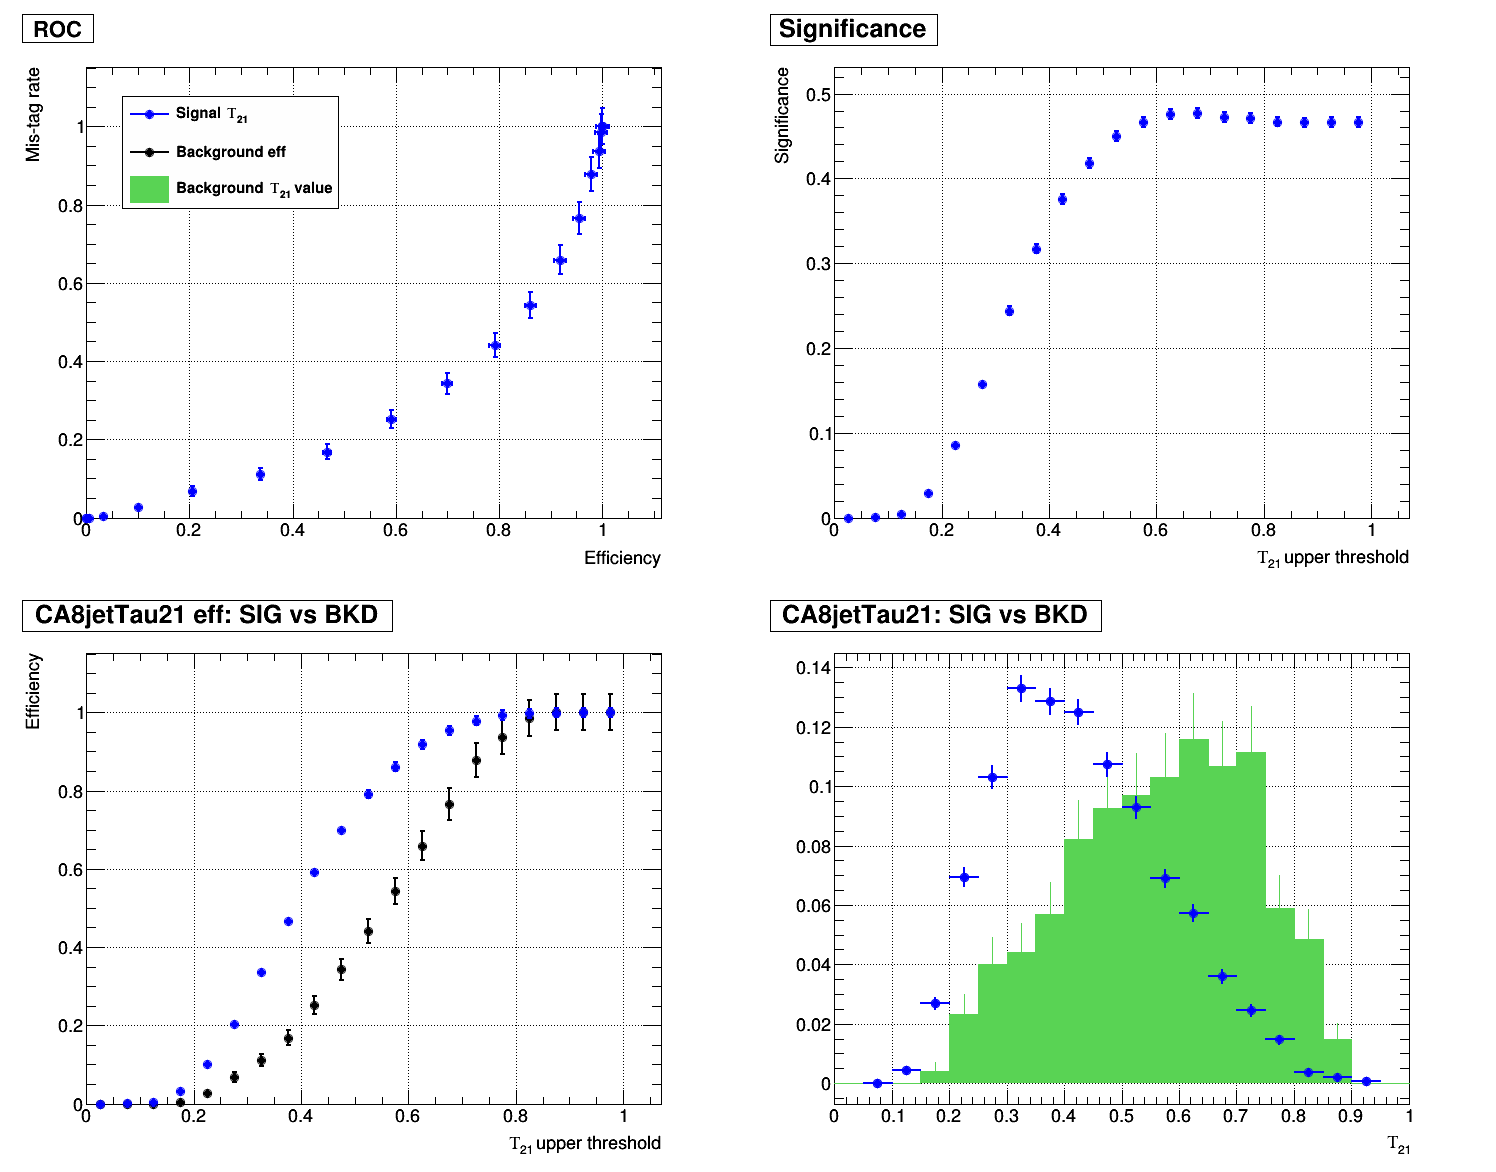
\includegraphics[width=0.8\linewidth]{tau21_M2000.png}}
  \caption{ZPrime mass 2000 GeV - upper left: ROC plot ; upper right: signal significance ; lower left: signal efficiency vs mistag rate ; lower rigth: compare $\tau_{21}$ distribution between MC signal and background}
  \label{fig:tau21_M2000}
\end{figure}



\subsection{b-tagging}

Jets are clustered from objects reconstructed by the particle-flow method. The b-tagging algorithm combines information from all subdetectors to create a consistent set of reconstructed particles for each event.

\noindent
$\bullet$ Combined Secondary Vertex (CSV): secondary vertices and track-based lifetime information are used to build a likelihood-based discriminator to distinguish between jets from b-quarks and those from charm or light quarks and gluons.

To identify Higgs jets arising from the shower and hadronization of two collimated b quarks, we apply b tagging either on the two subjets or the fat jet , based on the angular separation of the two subjets, which is recommended by BTV-13-001.

Subjet b-tagging:\\
\noindent
   $\bullet$ if $\Delta R$ between the CA8 subjets is bigger than 0.3: both subjets must pass the CSV Loose working point. \\
   $\bullet$ if $\Delta R$ between the CA8 subjets is smaller than 0.3: require the fat CA8 jet to pass the CSV Loose working point. \\

Here we study the efficiency and significance of b-tagging CSV, we use the same definition as our study in optimizing $\tau_{21}$. Figure~\ref{fig:btag_M1500} shows the result of 1500 GeV mass point.



\begin{figure}[H] % Image
  \center{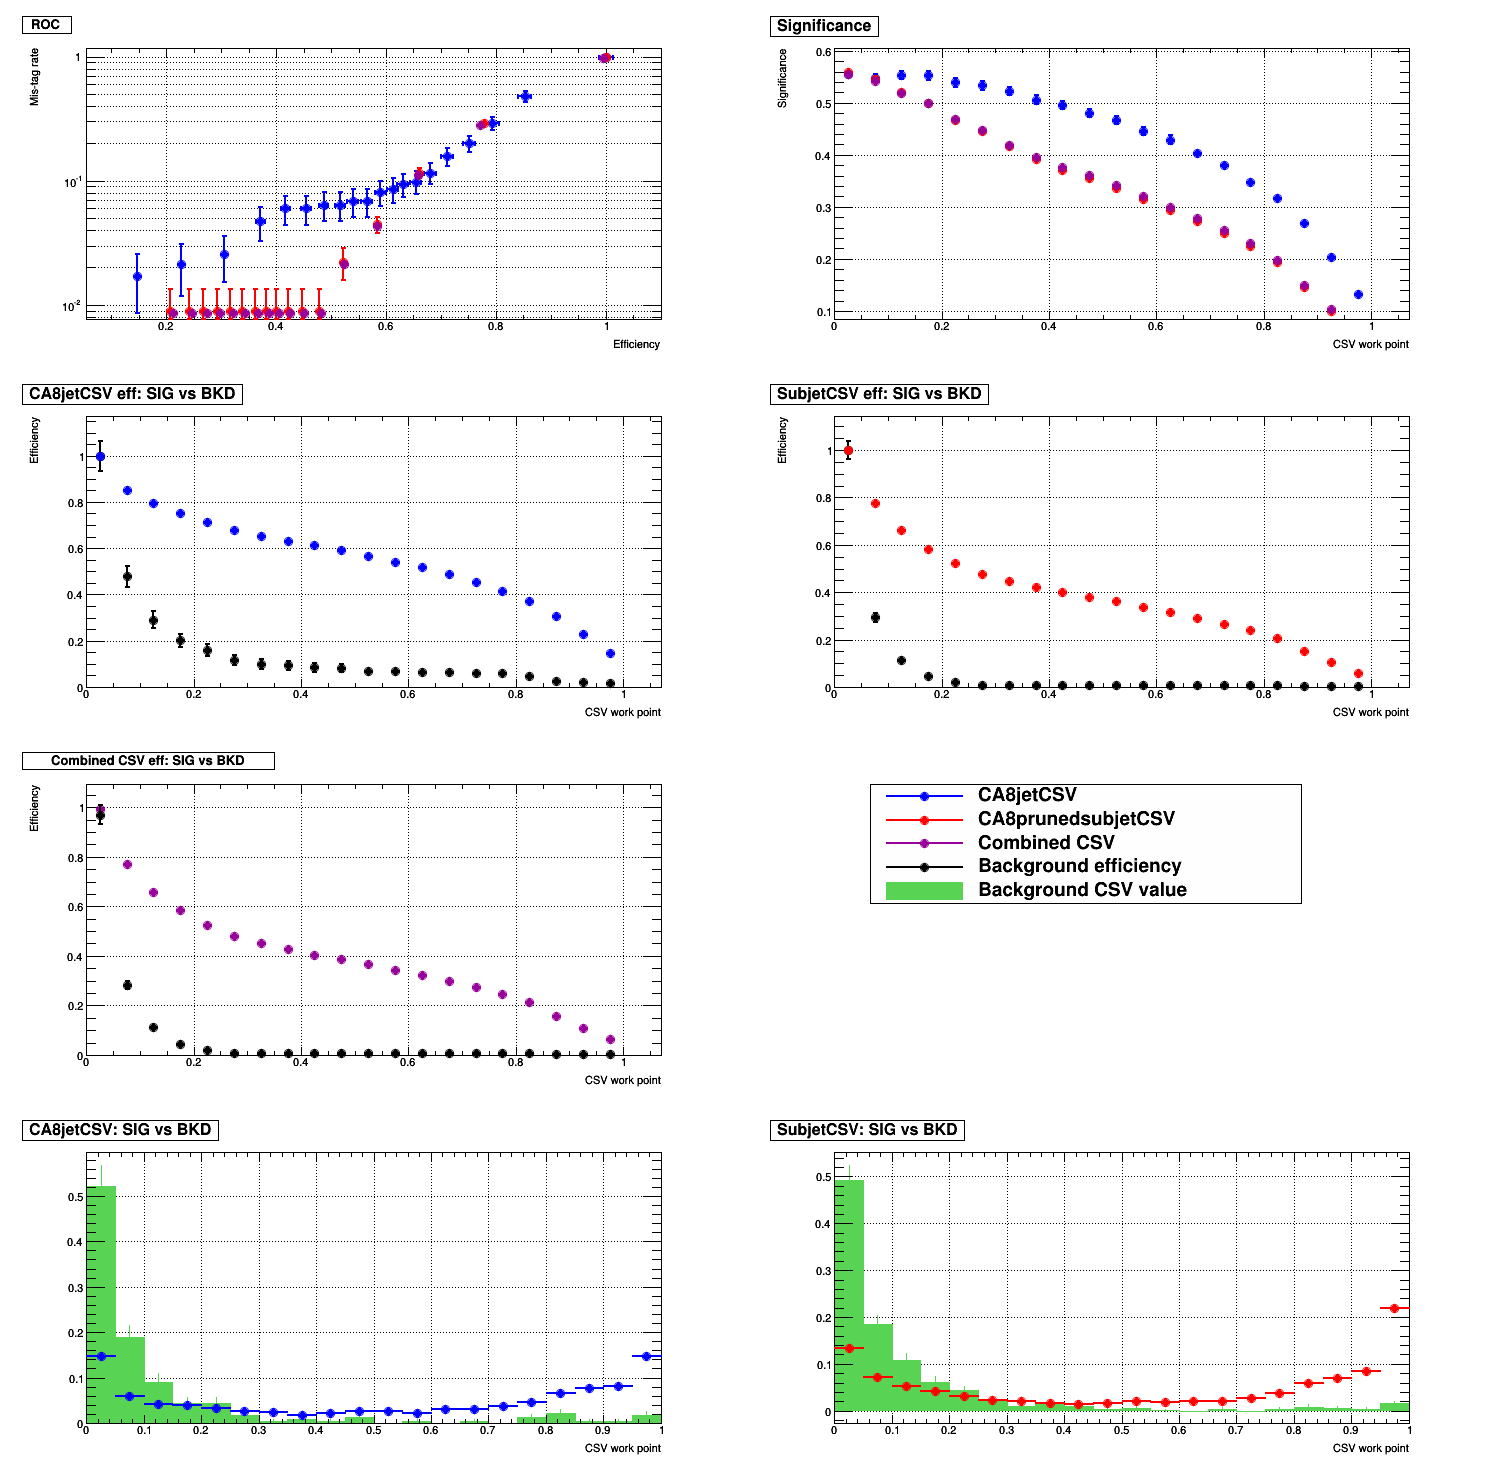
\includegraphics[width=0.8\linewidth]{btag_M1500.png}}
  \caption{Mis-tag rate versus efficiency, significance, background and signal efficiency plots. The definition of combined CSV efficiency: numerator is the sum of two terms, number of CA8 fatjet pass certain CSV cut if $\Delta R<0.3$, number of subjet pass certain CSV cut if $\Delta R>0.3$, and denominator is the number of CA8jets passing selections. The fatjet efficiency(number of CA8 fatjets passing CSV cut divided by number of all selected jets) at CSV Loose working point(0.244) is about 70\% while mistag rate is about 10\%. Subjet efficiency(require $\Delta R_{subjets} <0.3$, number of two subjets passing CSV cut events divided by number of all subjet events) after CSVL cut is about 50\% while mistag rate is $<$ 10\%.}
  \label{fig:btag_M1500}
\end{figure}





\newpage

%----------------------------------------------------------------------------------------
%	MAJOR SECTION 3
%----------------------------------------------------------------------------------------

\section{Background Extrapolation} % Major section

The final aim of this analysis is to compare the predicted SM background with the observed data, it is important to elaborate a trustworthy strategy for the background estimation. Indeed, despite the good description of the event kinematics provided by the MC simulation, it is more advisable to minimize the dependence on the MC and develop a data driven strategy. 


\subsection{Sideband region} % Sub-section

We have already defined our signal region, we need now a sideband region to be used as a pure background control region, where we can check the correct behaviour of the MC (background) simulation compared to the observed data. 

Indeed, such a control region should contain a pure background sample and it is tipically defined as the sidebands of the signal region in the distribution of the main discriminating variables. In our case, we don't consider a right sideband of the pruned mass distribution, higher than 140 GeV, because of the poor statistics and the excessive contribution of $t\bar{t}$ events.

At this point we have to select wisely an adequate left sideband region. The two possible selection of the left sideband regions are:

\noindent
1. thin sideband: [50, 70] GeV \\
2. large sideband: [50, 110] GeV 

The weakness of the former choice is the lack of statistics at high masses, due to the small range and low value of the sideband considered. In fact, although the background is exponentially distributed in term of the invariant ZH mass, the jet mass and the final invariant mass are strongly correlated and the extension of the sideband up to 110 GeV largely helps the increasing of the population of the high invariant mass region.


\subsection{$\alpha$ ratio} % Sub-section

In order to estimate the final background, we consider the $m_{ZH}$ MC mass spectrum in the signal and sideband region. A ratio $\alpha$($m_{ZH}$) of the two is created. This $\alpha$ factor allows a prediction of the mass spectrum in the signal region starting from the measured distribution in the sideband. Under the assumption that this estrapolation from the sideband to the signal region works in the same way both for data and MC, we can estimate the final background distribution by multipling the $m_{ZH}$ mass spectrum observed in the sideband by this $\alpha$ ratio:

$N_{bkd}^{data}(m_{ZH}) = N_{sb}^{data}(m_{ZH})\times \frac{N^{MC}_{bkd}(m_{ZH})}{N^{MC}_{sb}(m_{ZH})}= N_{sb}^{data}(m_{ZH})\times \alpha (m_{ZH})$


We divide the spectrum in 14 not uniform width bins, as shown in Table~\ref{tab:bin}, accordingly to the decreasing statistics in the high mass tail.

The MC background distribution in the signal region is used to explore the range where the invariant mass is well described by an exponential function.

\begin{center}
  \begin{tabular}{ c | c }
    \hline
    \bf Bin & \bf GeV \\
    \hline
    \hline
    1 & [680, 720] \\
    2 & [720, 760] \\
    3 & [760, 800] \\
    4 & [800, 840] \\
    5 & [840, 920] \\
    6 & [920, 1000] \\
    7 & [1000, 1100] \\
    8 & [1100, 1250] \\
    9 & [1250, 1400] \\
    10 & [1400, 1600] \\
    11 & [1600, 1800] \\
    12 & [1800, 2000] \\
    13 & [2000, 2200] \\
    14 & [2200, 2400] \\
    \hline
  \end{tabular}
  \captionof{table}{Binning of the X invariant mass range.}
  \label{tab:bin}
\end{center}

Finally, we can take the product of the $\alpha$ ratio obtained (fig.~\ref{fig:alpha}) and the sideband data $M_x$ to get the prediction of background in the signal region.

\begin{figure}[H] % Image
  \center{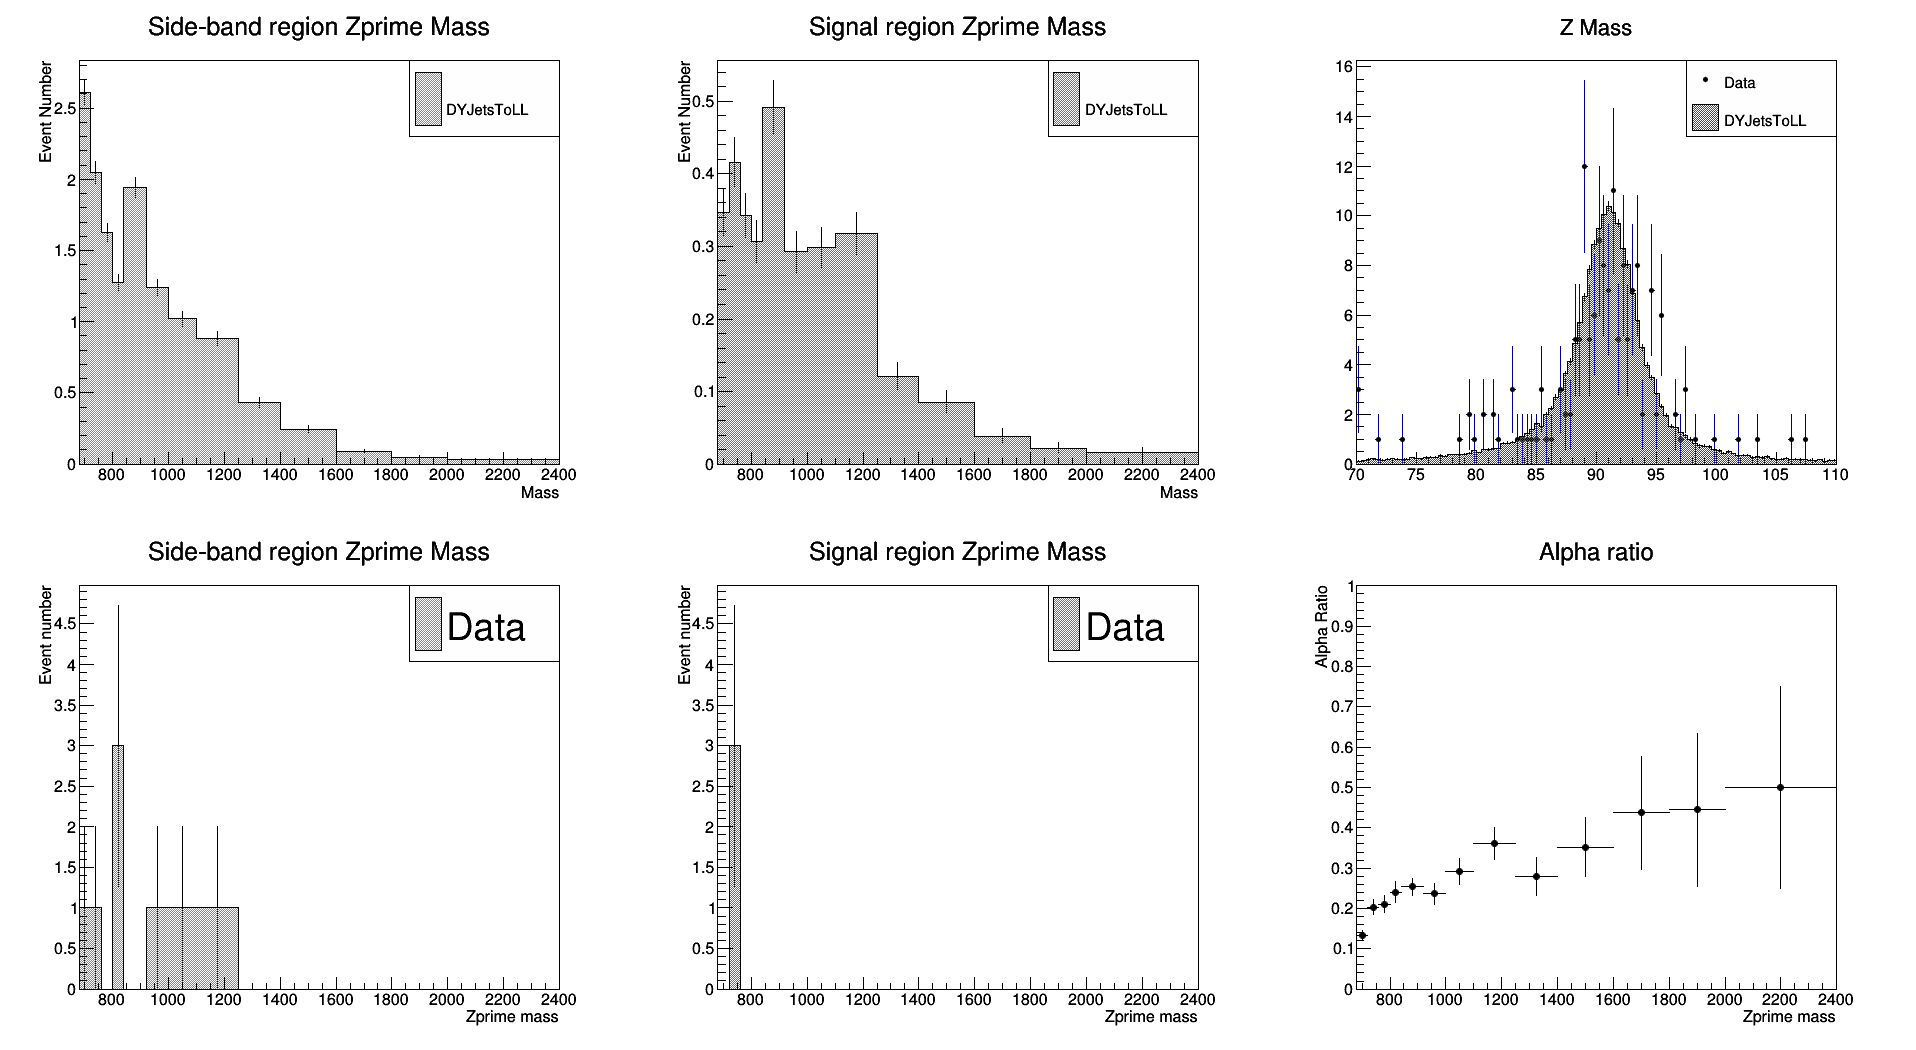
\includegraphics[width=1\linewidth]{backgroundEstimation.png}}
  \caption{MC $m_{ZH}$ observed distribution in the sideband region (top left) and in the signal region (top middle); Data $m_{ZH}$ observed distribution in the sideband region (bottom left) and in the signal region (bottom middle). Bottom right: $\alpha$ ($m_{ZH}$) ratio computation.}
  \label{fig:alpha}
\end{figure}




%----------------------------------------------------------------------------------------
%	CONCLUSION
%----------------------------------------------------------------------------------------

\section{Future Progress} % Major section

The current result of background estimation did not include b-tagging CSVL cut. Re-evaluate $\alpha$ ratio after applying btagging will be done in the near future and obtain background prediction. After that, we will estimate systematic uncertainty and the final goal is to set limit.




\newpage


\section{Validation of HVT model and Abelian Higgs model}

We will no longer use Abelian Higgs model and old version matrix element generator in our future analysis stage. Although we still need to do some validations between the new model and old one, theoretically these two models have same decay channels and kinematics of their decay products. We do the following comparison. First, we compare the new model using different version of generators Figure~\ref{fig:oldnewgen} to prove there's no inconsistent between versions of generators. Later we check using the same generator but the different models. Figure~\ref{fig:width} We see good agreement between models, note that the black distribution is the control sample which is set narrower ZPrime decay width.


\begin{figure}[H] % Image                                                                           
  \center{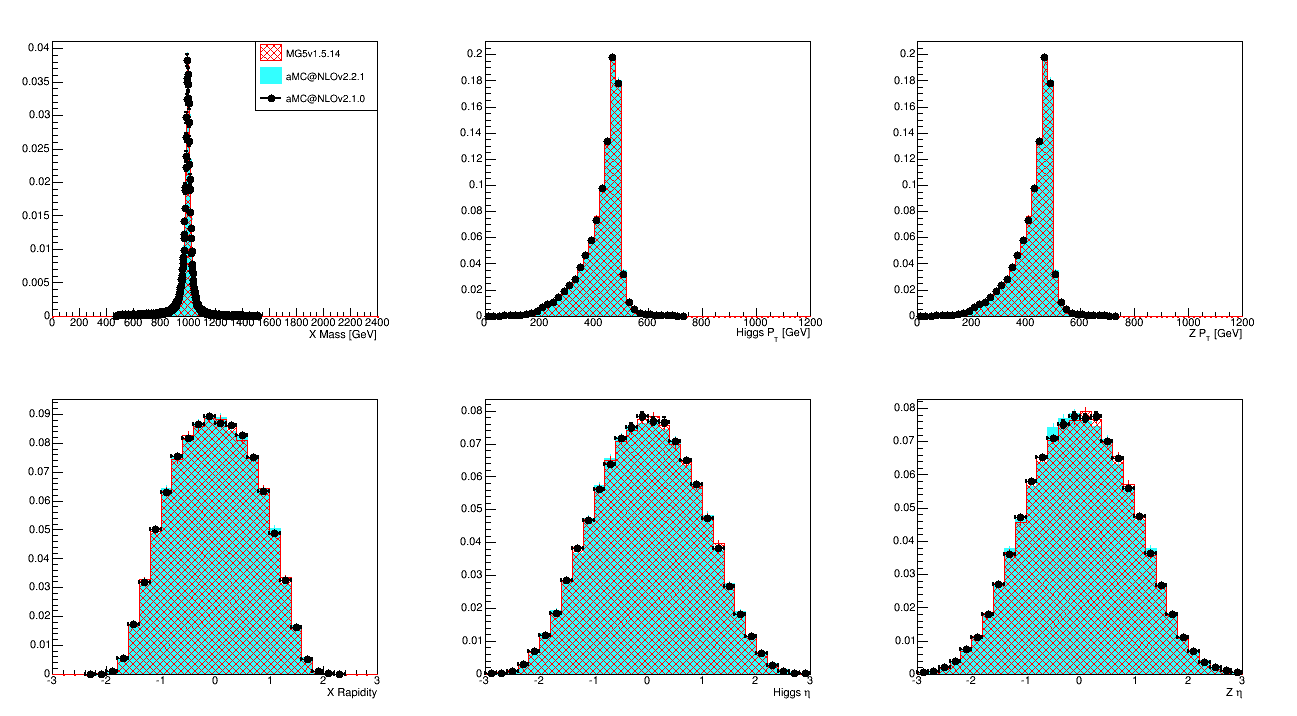
\includegraphics[width=0.8\linewidth]{oldnewgen.png}}
  \caption{Basic kinematic distributions comparison plots of ZPrime, Higgs and Z boson. Here we set all the parameters the same but different version of MadGraph. The results shows there's no different between 1.5.14, aMC@NLOv2.2.1 and 2.1.0.}
  \label{fig:oldnewgen}
\end{figure}

\begin{figure}[H] % Image                                                                           
  \center{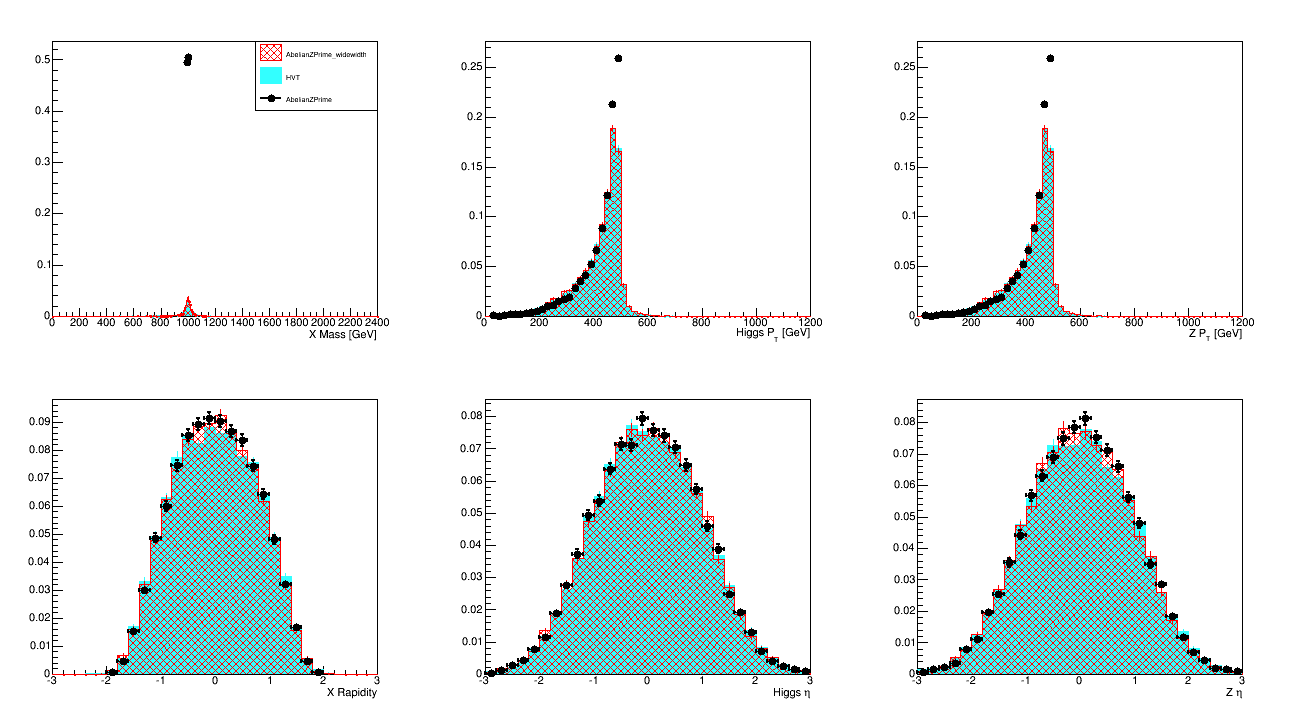
\includegraphics[width=0.8\linewidth]{width.png}}
  \caption{In this figure, the Madgraph version we use is 1.5.14. The results shows good agreement between the two models. The black distribution is the control sample which is set narrower ZPrime decay width, we also comfirm that change the value of ZPrime decay width do affect the kinematics(Higgs and Z boson $P_{T}$).}
  \label{fig:width}
\end{figure}




\section{Validation of aMC@NLO}

In this section I will show my work in the matrix element generator group. This study is aim to compare the LO and NLO of matrix element generator we use: aMC@NLO after PYTHIA8 parton shower. The samples we use is listed below.

\noindent
$\bullet$ Drell-Yan + 0jet, LO \\
$\bullet$ Drell-Yan + 0jet, NLO \\
$\bullet$ Drell-Yan + 0-1jet, LO \\
$\bullet$ Drell-Yan + 0-1jet, NLO FXFX merging \\

Note that they're all 5 flavour samples and force Z decay into two leptons. We compare their kinematics distribution, jet multiplicity and Z boson mass. Figure~\ref{fig:MG5_Z} Figure~\ref{fig:MG5_Jet} Figure~\ref{fig:MG5_Rap}

Theoretically, jet and Z kinematics should be the same after parton shower. About jet multiplicity, we expect that the two 0-1jet samples have larger events number in high multiplicity region due to one additional jet in matrix element level.



\begin{figure}[H] % Image                                                                           
  \center{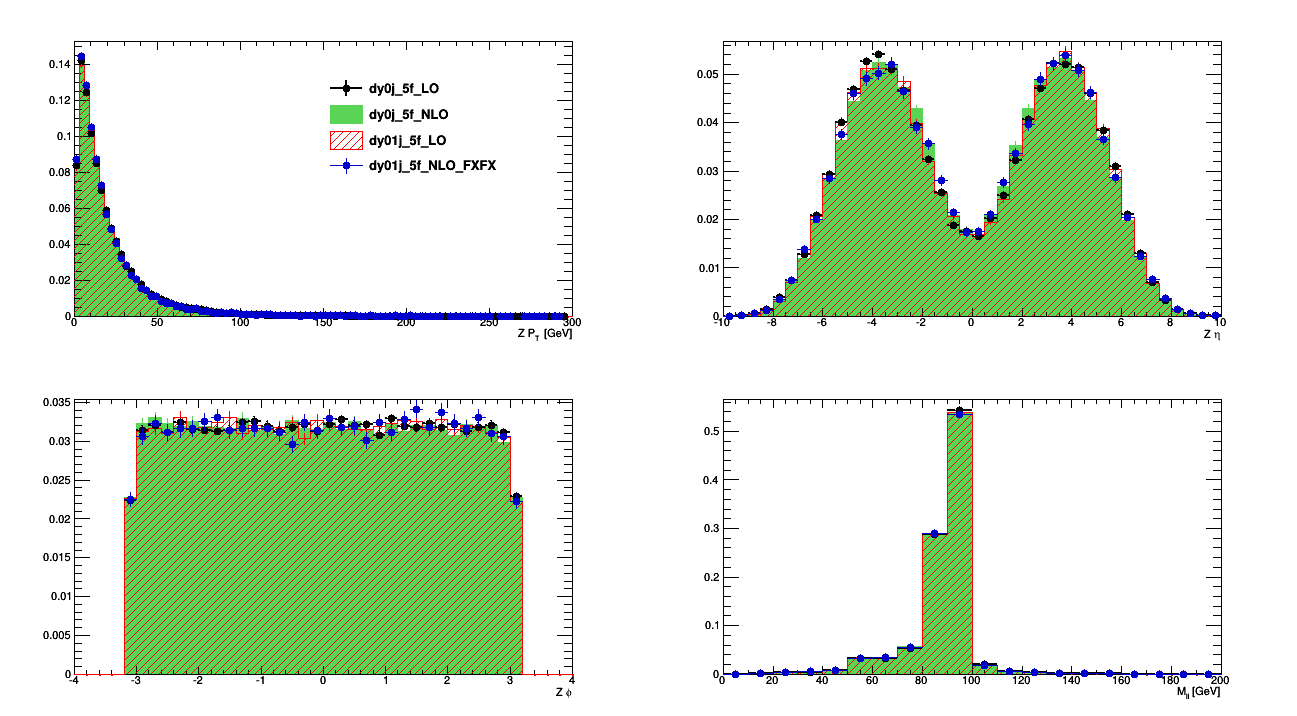
\includegraphics[width=0.8\linewidth]{MG5_Z.png}}
  \caption{Z boson kinematic distributions and di-lepton mass spectrum, the four samples are consistent.}
  \label{fig:MG5_Z}
\end{figure}


\begin{figure}[H] % Image                                                                           
  \center{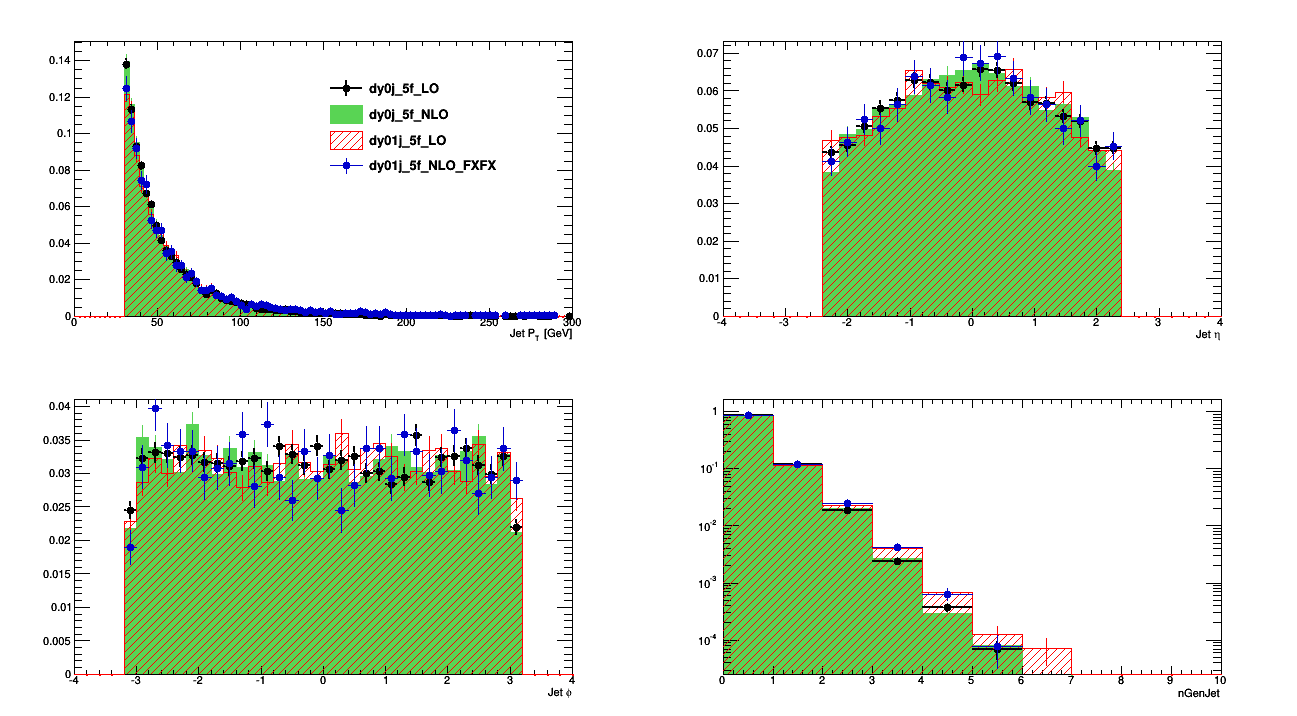
\includegraphics[width=0.8\linewidth]{MG5_jet.png}}
  \caption{Jet kinematics and multiplicity. Jet multiplicity is consistent for the first two jets region. For $>$2 jets region, the number of events of 0-1jet samples are more than others, as we expected, due to one additional jet in matrix element level of the two 0-1jet samples.}
  \label{fig:MG5_Jet}
\end{figure}


\begin{figure}[H] % Image                                                                           
  \center{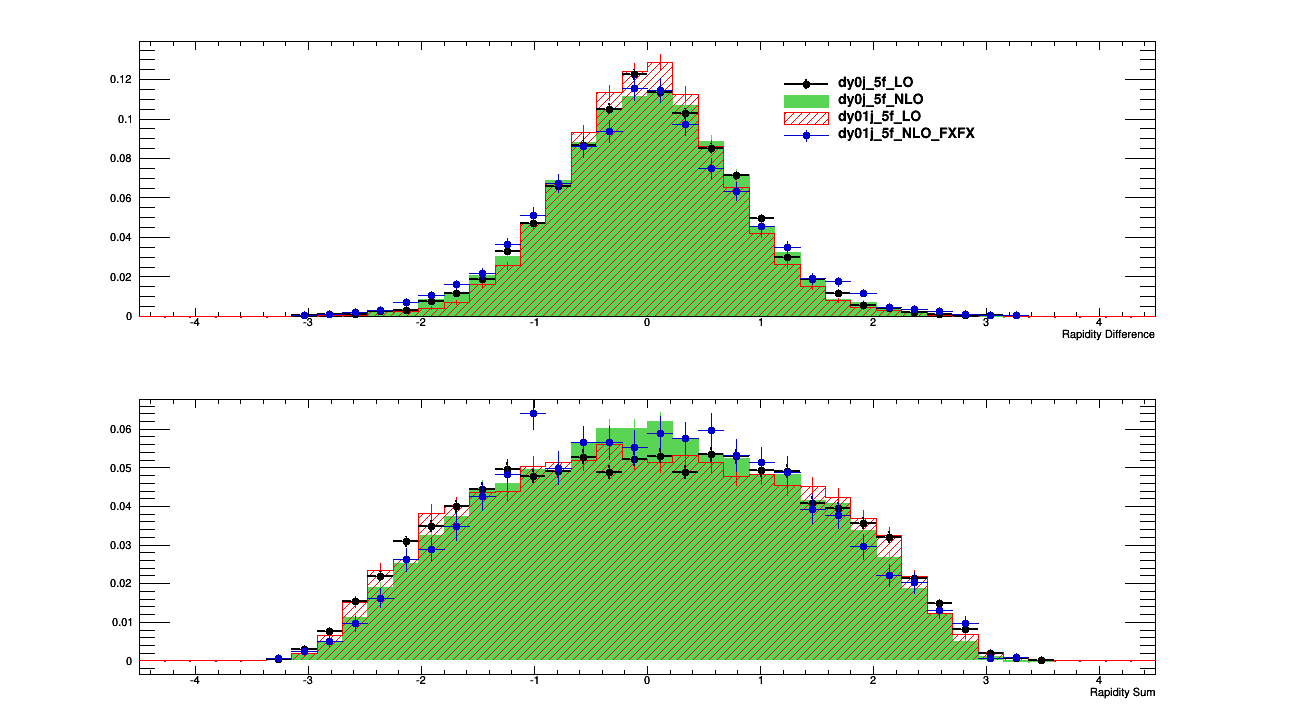
\includegraphics[width=0.8\linewidth]{MG5_Rap.png}}
  \caption{Rapidity sum and difference. The definition of rapidity sum is $\frac{Z_{y}+Jet_{y}}{2}$, for rapidity difference is $\frac{Z_{y}-Jet_{y}}{2}$. The distribution is consistent if considering uncerntainty.}
  \label{fig:MG5_Rap}
\end{figure}





\newpage
%----------------------------------------------------------------------------------------
%	BIBLIOGRAPHY
%----------------------------------------------------------------------------------------

\begin{thebibliography}{9} % Bibliography - this is intentionally simple in this template

\bibitem{Erdos01} Andrea Mauri, \emph{Search for new exotic resonances in semileptonic ZH final state at CMS}, 3 February 2014.
\bibitem{Erdos02} Duccio Pappadopulo, Andrea Thamm, Riccardo Torre, Andrea Wulzer, \emph{Heavy Vector Triplets: Bridging Theory and Data}, 9 October 2014.
\bibitem{Erdos03} The CMS Collaboration, \emph{Performance of b tagging at $\sqrt{s}$ = 8 TeV in multijet, $\bar{t}t$ and boosted topology events}, BTV-13-001, 15 August 2013.


\end{thebibliography}

%----------------------------------------------------------------------------------------

\end{document}
